\documentclass[../../main.tex]{subfiles}

\graphicspath{{\subfix{../../immagini/}}}

\begin{document}
Come illustrato nei paragrafi precedenti i modelli basano la loro efficacia sul valore dei loro parametri (per questo motivo rientrano nella categoria dei modelli parametrici), perciò è necessario disporre di tecniche che permettano di ottimizzare, il valore di questi parametri. Egual importanza hanno però anche i parametri del modello scelti a priori e non aggiornabili durante l'addestramento, che prendono il nome di iperparametri, un semplice esempio di iperparametro è il numero di neuroni in uno strato nascosto di una rete feedforward; la scelta ad esempio di un numero di neuroni molto basso potrebbe portare ad avere un modello non in grado, anche dopo l'addestramento, di rappresentare in modo soddisfacente la funzione obiettivo.

\begin{figure}[H]
    \centering
    \begin{subfigure}[t]{0.30\textwidth}
        \centering
        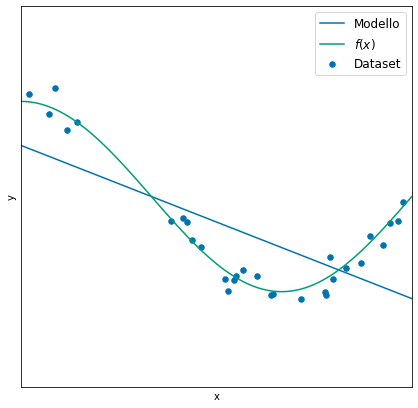
\includegraphics[width=\textwidth]{immagini/4_2/4_2_3/under.png}
        \caption{}
        \label{fig:underfitting}
    \end{subfigure}
    \begin{subfigure}[t]{0.30\textwidth}
        \centering
        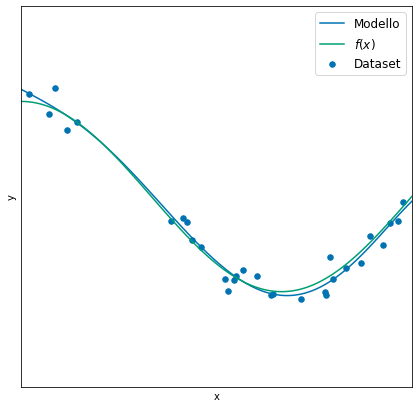
\includegraphics[width=\textwidth]{immagini/4_2/4_2_3/good.png}
        \caption{}
        \label{fig:goodfitting}
    \end{subfigure}
    \begin{subfigure}[t]{0.30\textwidth}
        \centering
        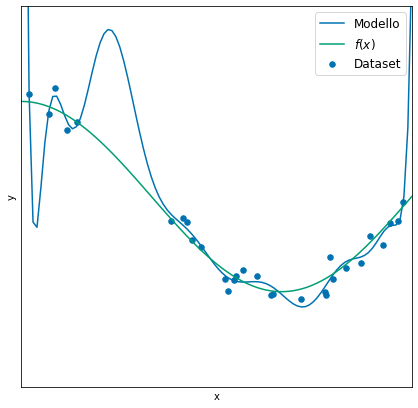
\includegraphics[width=\textwidth]{immagini/4_2/4_2_3/over.png}
        \caption{}
        \label{fig:overfitting}
    \end{subfigure}
    \caption{Esempi di modelli addestrati. (a) Mostra un esempio di underfitting: il modello dopo l'addestramento non è in grado di descrivere bene neanche i dati d'addestramento. (b) Mostra un esempio di un buon modello, in grado di approssimare correttamente i dati d'addestramento e di fornire un buon grado di generalizzazione. (c) Mostra un esempio di overfitting: il modello dopo l'addestramento è in grado di descrivere correttamente i dati d'addestramento, ma non è in grado di generalizzare.}
\end{figure}

Più nello specifico questo introduce il problema di dover bilanciare tra \textit{bias} e \textit{varianza} di un modello: un bias ridotto indica che il modello è in grado di descrivere bene la distribuzione di dati d'addestramento, viceversa un bias elevato implica un modello non in grado di descrivere neanche il training set, in questo caso parlo di \textit{underfitting} (figura \ref{fig:underfitting}). La varianza è invece legata alla capacità del modello di generalizzare, quindi di descrivere dati non osservati durante l'addestramento, in caso di alta varianza il modello ha semplicemente imparato a `memoria' i dati dell'insieme d'addestramento, ma non è in grado di generalizzare, si quindi parla di \textit{overfitting} (figura \ref{fig:overfitting}).

Scegliere modelli troppo complessi può quindi portare ad avere un bias basso, ma una varianza molto alta, viceversa modelli troppo semplici potrebbero portare ad avere una varianza contenuta, ma un bias elevato, in questo senso l'obiettivo è di trovare un giusto compromesso tra bias e varianza selezionando iperparametri, e una classe del modello, adeguati. La figura \ref{fig:goodfitting} mostra un modello in grado di descrivere bene sia i gli esempi dell'insieme d'addestramento che eventuali nuovi esempi.

Non esistono regole che permettono di ricavare il modello migliore in questo senso, spesso si procede quindi analizzando diversi modelli con diverse configurazioni; esistono diverse metriche per quantificare le performance di un modello, quelle utilizzate negli esperimenti vengono descritte nel paragrafo \ref{sec:metrichevalutazione}.
\end{document}